The tracking sub-detectors are responsible for registering spacial coordinates of charged particles.
The coordinates from multiple layers of tracking sub-systems are processed by the tracking algorithms
to produce {\it tracks}, which are objects representing the trajectory of a charged particle. There are
three distinct tracking sub-detectors in \lhcb shown in \figref{lhcb_detector_cross_section}; Closest to the interaction point is
the {\it VErtex LOcator}, \velo, then just before the \lhcb magnet is the {\it Tracker Turicensis}, \ttracker,
and  lastly the T stations. The latter consists of the {\it Inner Tracker}, \intr, and the {\it Outer Tracker}, \ot,
covering the area after the \lhcb magnet. There are several track types that are {\it reconstructed} by
the tracking algorithms, depending on which of the tracking sub-detectors provided information to produce
the track object. The various track types are shown in \figref{track_types}. The most common tracks used
are {\it Long} which have the best momentum resolution.
% The overall reconstruction efficiency of Long
% tracks is $\sim 96\%$ and it is estimated with the so called {\it tag and probe} method \cite{Aaij:1748269}.

\begin{figure}[t]
  \centering
  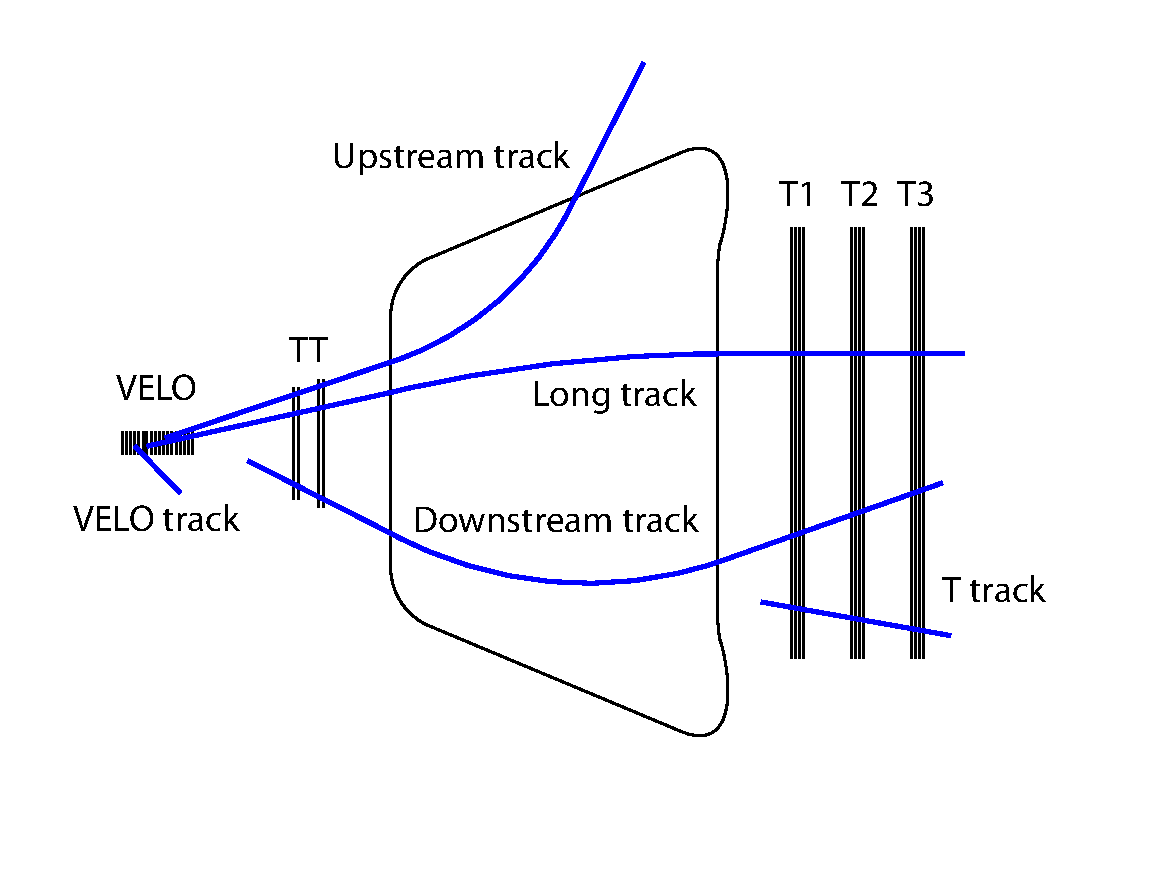
\includegraphics[width=0.7\textwidth]{Figures/Chapter2/trackTypesRunIAndII}
  \caption{Various track types in \lhcb.}
  \label{track_types}
\end{figure}

A charged particle that traverses the \lhcb magnet is deflected. The amount of deflection is inversely proportional
to its momentum, which is exploited by tracking algorithms to estimate the momentum of a track. The relative
momentum resolution of the tracking system, shown in \figref{det_deltappvp}, is $\nicefrac{\Delta p}{p} \sim 0.5 \%$
for low momentum tracks and up to $1\%$ for 200\gevc momentum tracks.

Measuring the mass of a particle, like the \Bs meson, is achieved by reconstructing particles in order to build a
complete cascade of particle decays (also referred to as {\it decay channel}). The mass measurement precision varies depending
on the specific decay channel. Two body \B decays including a \jpsi have a very precise mass resolution of about
$8 \mevcc$. On the other hand decay channels including neutral particles, \ie $\BsPhiGam$, have a worse
resolution of about $100 \mevcc$. Note that neutral particles are not detected by the tracking system.
Instead the calorimetry system, introduced in \secref{det_calo}, is responsible for identifying and
reconstructing these type of particles.

\begin{figure}[t]
  \centering
  \begin{subfigure}{0.5\textwidth}
    \raggedright
    \includegraphics[width=\textwidth]{Figures/Chapter2/dppVsp-crop-cmyk}
    \caption{}
    \label{det_deltappvp}
  \end{subfigure}%
  \hfill%
  \begin{subfigure}{0.5\textwidth}
    \raggedleft
    \includegraphics[width=\textwidth]{Figures/Chapter2/DataResXY_1PV_2012-crop-cmyk.pdf}
    \caption{}
    \label{det_velo_pv_res}
  \end{subfigure}
  \caption{Tracking performance plots. (A): Relative Long track momentum resolution as a function of momentum.
          (B): Primary vertex resolutions versus the number of tracks present in the vertex, $N$. The gray area
          indicates the distribution of $N$.}
  \label{det_velo_perf}
\end{figure}

Many important analyses performed with the \lhcb detector rely on measuring the {\it decay time} of a particle,
like the \Bs meson, which is the time interval between the production and decay of a particle.
This particular measurement requires knowledge of the {\it flight distance}, which is the
distance between the point were the two protons collided, called {\it Primary Vertex} (PV) and the point were the
\Bs, in that case, decayed. This latter point is called {\it Secondary Vertex} (SV). The decay time is the actual
quantity that a typical {\it lifetime dependent} analysis, \eg \BsJpsiPhi, requires.
The \velo sub-detector was designed for optimum spacial resolution by placing the \velo sensors as close to the beam
as possible, $\sim 8 \mm$. The \velo sensors are the closest detector element along the entire \lhc beam.
The PV position resolution depends on the number of tracks used to build the vertex and can
be seen in \figref{det_velo_pv_res}. The average decay time resolution measured with \BsJpsiPhi data is $\sim 45\fs$,
which enables the \phis measurement discussed in \secref{measuring_phis}.

Lastly, a big part of the \lhcb physics program includes muons. The muon system consists of {\it Multi Wire Proportional Chambers}
(MWPC). It is positioned after the calorimeters, with the exception of the first muon station, M1.
Note that muons can penetrate through a large volume of lead, like the one present in the calorimeter system,
without decaying or loosing much energy. There are five muon stations in total; Each station is divided in four concentric
regions. The granularity\footnote{In this context granularity is the distance between the wires of the MWPC.}
of each station becomes progressively smaller as one moves towards the inner regions which are closer to the beam.
This is done to account for the increasing particle density. This way the special resolution is higher exactly where
it is needed. The horizontal coordinate hit resolution in all regions is superior compared to the vertical coordinate.
Given that the \lhcb magnet bends charged particles in the horizontal plane, the position resolution in this plane
is crucial for the momentum measurement. As a result the (horizontal,vertical) resolution varies from $(4,10)\mm$ to
$(150,180)\mm$ respectively for the inner M1 region and the outer M5 region. Details on the overall muon system
efficiency can be found in \cite{AlvesJr:1492807}.
